The \SwissRangerCam{} class and its components are very similar to the classes that describe a color 
camera in \RD{}. This proves that the system can represent cameras following a similar core structure. Like 
\ColorCam{}, the \SwissRangerCam{} class extends \Camera{}. In this case it represents a SwissRanger
sensor, a 3D time-of-flight camera produced by Mesa Imaging \cite{SR4000Manual}. The SwissRanger 
can capture depth information (z-coordinates) from a scene, as well as x-coordinates and y-coordinates for 
each of the depth points. Associated with this data is the amplitude and the confidence map, which provide
measurements of the quality of the acquired data. 

In the representation, the SwissRanger can be connected directly to the computer running the system, or it 
can be connected to some other device that sends the images over the network to \RD{}. This versatility is 
provided through the \SwissRangerReceiver{} class. While the SwissRanger receiver is in charge of acquiring 
and handling the images from the camera, the SwissRanger camera provides access to the image buffers, 
the image views, and the camera calibration tool, as well as the implementation of all abstract methods 
defined by the \Camera{} class. Furthermore, it contains the information about the modulation frequency 
on which the SwissRanger is running, and static methods to create visualizations for the depth and amplitude 
data. Table \ref{swissrangercammethods} lists the methods that the SwissRanger class adds to the base 
camera representation.

\begin{table}[ht]
\caption{Public methods in the \SwissRangerCam{} class}
\begin{center}
\begin{tabular}{| l |}
	\hline 
	\multicolumn{1}{| c |}{\SwissRangerCam{}} \\
	\multicolumn{1}{| c |}{{\small \texttt{extends} \Camera{}}} \\
	\hline \hline
	\texttt{getDepth} \\
	\texttt{getAmplitude} \\
	\texttt{getX} \\
	\texttt{getY} \\
	\texttt{getConfidenceMap} \\
	\texttt{getDepthDisplay} \\
	\texttt{getAmplitudeDisplay} \\
	\texttt{getDepthView} \\
	\texttt{getAmplitudeView} \\
	\texttt{getCalibrationTool} \\
	\texttt{getModulationFrequency} \\
	\texttt{createDisplays} \\
	\texttt{threshold} \\
	\texttt{toMeters} \\
	\hline
\end{tabular}
\end{center}
\label{swissrangercammethods}
\end{table}

There are two ways of accessing the image data captured by the SwissRanger. One way is through the 
camera object's internal image buffers, which store copies of the last grabbed images. The depth data
is obtained by calling the \texttt{get\-Depth} method, and the amplitude data is obtained by calling 
\texttt{get\-Am\-pli\-tude}. The x-coordinate, y-coordinate, and confidence map data are obtained by calling
\texttt{getX}, \texttt{getY}, and \texttt{get\-Con\-fi\-dence\-Map}, respectively.

The second way takes advantage of \RD{}'s intra-application communication system and consists of 
subscribing to the data objects of type \SwissRangerCamData{} through the \DataHandler{} interface. 
A SwissRanger data object contains the same number of image buffers as described before, each with a 
copy of the last grabbed image. The \texttt{han\-dle\-Da\-ta} method of the data handler receives these data 
objects. 

Similar to the \ColorCam{} class, when the \texttt{grab\-Im\-age} method returns successfully the acquired 
images are stored in the internal image buffers and then are published through the \DataProvider{} interface. 
Accessing the images directly from the image buffers avoids the overhead of going through the data 
dispatcher mechanism and allows the user to process the images right after they are grabbed. However, 
receiving the images published through the data dispatcher simplifies the communication between \RD{} 
applications. 

Furthermore, the \SwissRangerCam{} class also adds a second version of the \texttt{grab\-Im\-age} method.
The reason for this method becomes clearer now. A Firewire color camera could be synchronized with a 
SwissRanger, but differences in the devices and their capturing mechanisms might not give the user the 
same capturing frame rate nor the same timestamp for images captured at the same time. Since this second 
version of the \texttt{grab\-Im\-age} method takes as input a desired timestamp for the grabbed image, it is 
possible to get a timestamp from one of the cameras and retrieve the closest corresponding image from the 
second camera taking into account a timestamp offset.

The \SwissRangerCam{} class provides the option of displaying visualizations for the depth image stream 
and the amplitude image stream. The methods \texttt{get\-Depth\-Dis\-play} and 
\texttt{get\-Am\-pli\-tude\-Dis\-play} return image buffers with BGR color model and \texttt{BYTE} pixel depth 
containing the image data of the visualizations. These image buffers are linked to \ImageView{} objects and 
are obtained through the \texttt{get\-Depth\-View} and \texttt{get\-Am\-pli\-tudeView} methods. The method 
\texttt{cre\-ate\-Dis\-plays} is used to create the visualizations from the raw depth and amplitude data.

The \CalibrationTool{} class is again used to provide the methods that perform camera calibration and retrieve
the camera's parameters. Since the amplitude image is visually close to a grayscale image, the calibration tool 
object is linked to the internal amplitude image buffer of the \SwissRangerCam{} instance. The user can 
access this object through the \texttt{get\-Cal\-i\-bra\-tion\-Tool} method, and then calibrate the camera by 
using the methods discussed in Section \ref{calibrationtool}.

The following sections present and discuss the modules that make up the \SwissRangerCam{} class. Figure 
\ref{swissrangercammoduledependency} shows a module dependency diagram that indicates how these 
classes are related to each other. 

\begin{figure}[t]
\begin{center}
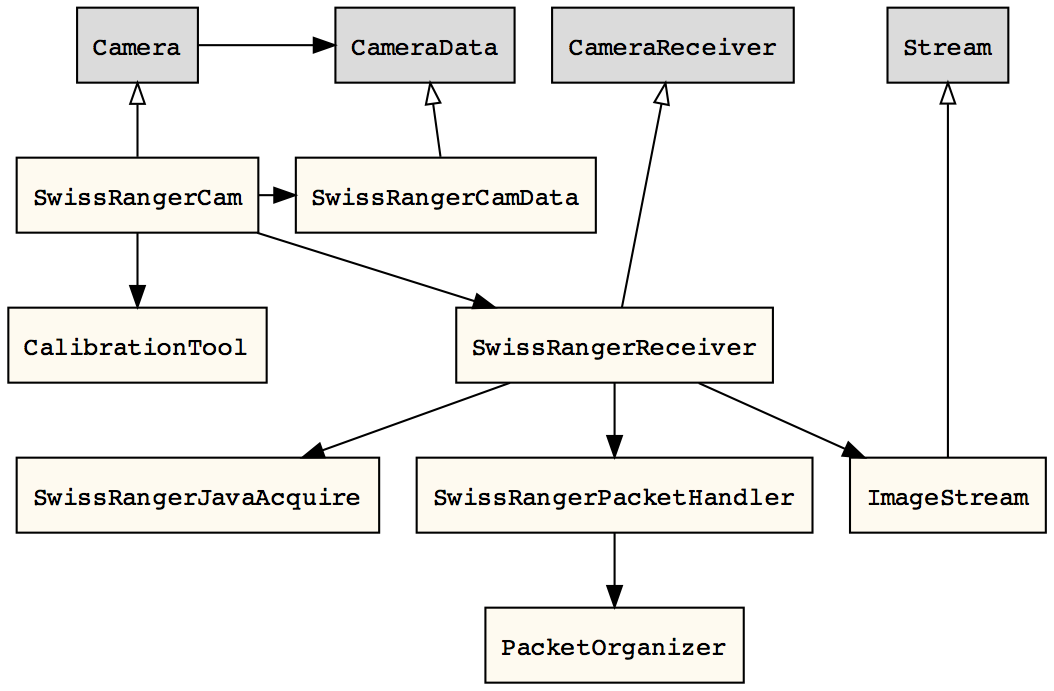
\includegraphics[width = 15cm]{SwissRangerCam.png}
%\digraph[scale=0.75]{SwissRangerCam}{
	graph [rankdir = "TB" margin = 0];
	node [shape = "box" style = "filled" fillcolor = "gainsboro" fontsize = "12" fontname = "Courier"];
		Camera CameraReceiver CameraData Stream;
	node [shape = "box" style = "filled" fillcolor = "floralwhite" fontsize = "12" fontname = "Courier"];
	{ rank = "source"; CameraReceiver Camera CameraData Stream;}
	{ rank = "same"; SwissRangerCam SwissRangerCamData;}
	{ rank = "same"; SwissRangerReceiver CalibrationTool;}
	{ rank = "same"; SwissRangerPacketHandler SwissRangerJavaAcquire ImageStream;}
	{ rank = "sink"; PacketOrganizer;}
	edge [arrowhead = "normal"];
	Camera -> CameraData;
	SwissRangerCam -> Camera [arrowhead = "empty"] ;
	SwissRangerCam -> SwissRangerCamData;
	SwissRangerCam -> SwissRangerReceiver ;
	SwissRangerCam -> CalibrationTool;
	SwissRangerCamData -> CameraData [arrowhead = "empty"];
	SwissRangerReceiver -> CameraReceiver [arrowhead = "empty"];
	SwissRangerReceiver -> SwissRangerPacketHandler;
	SwissRangerReceiver -> SwissRangerJavaAcquire;
	SwissRangerReceiver -> ImageStream;
	ImageStream -> Stream [arrowhead = "empty"];
	SwissRangerPacketHandler -> PacketOrganizer;
}
\caption[\SwissRangerCam{}'s module dependency diagram]{\SwissRangerCam{} module dependency 
diagram. Arcs with white arrows represent subtype relations (A $\vartriangleright$ B = A extends B) while 
arcs with black arrows represent implementation relations (A $\blacktriangleright$ B = A uses B). Gray 
rectangles represent abstract classes. The \ImageBuffer{} class is omitted from this diagram.}
\label{swissrangercammoduledependency}
\end{center}
\end{figure}
